\documentclass[a4paper,oneside,DIV=12,12pt,headings=normal]{scrartcl}

%%% Length calculations
\usepackage{calc}
%%%

%%% Support for color
\usepackage{xcolor}
\definecolor{lightblue}{HTML}{03A9F4}
\definecolor{red}{HTML}{F44336}
%%%

%%% Graphics inclusion
\usepackage{graphicx}
%%%

%%% Font selection
\usepackage{fontspec}

\setromanfont{STIX Two Text}[
	SmallCapsFeatures = {LetterSpace = 5},
]

\setsansfont{Source Sans Pro}[
]

\setmonofont{Source Code Pro}[
]
%%%

%%% Math settings
\usepackage{amsmath,unicode-math}
\setmathfont{STIX Two Math}

\usepackage{IEEEtrantools}
\usepackage{mleftright}
%%%

%%% Font settings for different KOMA Script elements
\setkomafont{pagenumber}{\rmfamily}
\setkomafont{disposition}{\rmfamily\bfseries}
%%%

%%% Typographic enhancements
\usepackage{microtype}
%%%

%%% Language-specific settings
\usepackage{polyglossia}
\setmainlanguage{ukrainian}
%%%

%%% List settings
\usepackage{enumitem}
\setlist[enumerate]{
	leftmargin = *,
}
%%%

%%% Captions
\usepackage{caption}
\usepackage{subcaption}

\DeclareCaptionLabelFormat{closing}{#2)}
\captionsetup[subtable]{labelformat = closing}
\captionsetup[subfigure]{labelformat = closing, position = auto}
%%%

%%% Tables
\usepackage{booktabs}
\usepackage{longtable}

\usepackage{multirow}

\usepackage{array}
\newcolumntype{v}[1]{>{\raggedright\arraybackslash\hspace{0pt}}p{#1}}
\newcolumntype{b}[1]{>{\centering\arraybackslash\hspace{0pt}}p{#1}}
\newcolumntype{n}[1]{>{\raggedleft\arraybackslash\hspace{0pt}}p{#1}}

\usepackage{kbordermatrix} % labeling array indices
%%%

%%% Floats on a single row
\usepackage{floatrow}
\newfloatcommand{capbtabbox}{table}[][\FBwidth]
%%%

%%% Links and hyperreferences
\usepackage{hyperref}
\hypersetup{
	colorlinks      = false,
	linkbordercolor = red,
	urlbordercolor  = lightblue,
	pdfborderstyle  = {/S/U/W 1.5},
}
%%%

%%% All caps
\newcommand{\allcaps}[1]{{\addfontfeatures{LetterSpace = 3}#1}}
%%%

%%% Ceiling function typesetting
\newcommand{\ceil}[1]{\mleft\lceil#1\mright\rceil}
%%%

\begin{document}
	\begin{titlepage}
	\centering
		Міністерство освіти і науки України\\
		Національний авіаційний університет\\
		Навчально-науковий інститут комп'ютерних інформаційних технологій\\
		Кафедра комп'ютеризованих систем управління

		\vspace*{\fill}

		Лабораторна робота №2\\
		з дисципліни «Архітектура комп'ютерів»\\
		на тему «Синтез керуючих автоматів з програмованою логікою»\\
		Варіант №4

		\vspace*{\fill}
		
		\begin{flushright}
			Виконав:\\
			студент ННІКІТ СП-225\\
			Клокун В.\,Д.\\
			Перевірив:\\
			Зіньков Ю.\,Г.
		\end{flushright}

		Київ 2018
    \end{titlepage}
	
	\section{Мета роботи}
		Закріплення теоретичних знань з синтезу керуючих автоматів із програмованою логікою.
		
	\section{Хід роботи}
		% \subsection{Побудова матриці сумісності мікрооперацій}
			Виконаємо кодування мікрооперацій. Для цього використаємо метод прямого включення. Спочатку з'ясуємо, які мікрооперації сумісні, а які ні. Для цього побудуємо матрицю сумісності~$S$ за таким принципом:
			\begin{IEEEeqnarray*}{l}
				S = \mleft[
				\begin{array}{*{4}{c}}
					0      & S_{12} & \dots  & S_{1M},\\
					S_{21} & 0      & \dots  & S_{1M},\\
					\vdots & \vdots & \ddots & \vdots\\
					S_{M1} & S_{12} & \dots  & 0
				\end{array}
				\mright],
				\quad
				S_{ij} =
				\begin{cases}
					1 \text{, якщо } y_i \text{ і }y_j \text{ сумісні,}\\
					0 \text{, якщо } y_i \text{ і }y_j \text{ несумісні}.
				\end{cases}
			\end{IEEEeqnarray*}
			В результаті отримали булеву симетричну матрицю сумісності~$S$:
			\begin{equation*}
				S = 
				% \kbordermatrix{*{17}{c} l}
				\kbordermatrix{
					% \begin{block}{*{17}{>{$\footnotesize}c<{$}} l}
						   & 1 & 2 & 3 & 4 & 5 & 6 & 7 & 8 & 9 & 10 & 11 & 12 & 13 & 14 & 15 & 16 & 17 \\
					% \end{block}
					% \begin{block}{(*{17}{c})>{$\footnotesize}l<{$}}
						1  & 0 & 1 & 0 & 0 & 0 & 0 & 0 & 0 & 0 & 0  & 0  & 0  & 0  & 0  & 0  & 0  & 1 \\
						2  & 1 & 0 & 1 & 0 & 0 & 0 & 0 & 0 & 0 & 0  & 0  & 0  & 1  & 0  & 0  & 0  & 1 \\
						3  & 0 & 1 & 0 & 0 & 0 & 0 & 0 & 0 & 0 & 0  & 0  & 1  & 0  & 0  & 0  & 0  & 1 \\
						4  & 0 & 0 & 0 & 0 & 1 & 0 & 0 & 0 & 0 & 0  & 0  & 0  & 0  & 0  & 0  & 0  & 0 \\
						5  & 0 & 0 & 0 & 1 & 0 & 0 & 0 & 0 & 0 & 0  & 0  & 0  & 0  & 0  & 0  & 0  & 0 \\
						6  & 0 & 0 & 0 & 0 & 0 & 0 & 1 & 0 & 0 & 0  & 0  & 0  & 0  & 0  & 0  & 0  & 0 \\
						7  & 0 & 0 & 0 & 0 & 0 & 1 & 0 & 1 & 0 & 0  & 0  & 0  & 0  & 0  & 0  & 0  & 0 \\
						8  & 0 & 0 & 0 & 0 & 0 & 0 & 1 & 0 & 0 & 0  & 0  & 0  & 0  & 0  & 0  & 0  & 0 \\
						9  & 0 & 0 & 0 & 0 & 0 & 0 & 0 & 0 & 0 & 0  & 0  & 0  & 0  & 0  & 1  & 0  & 0 \\
						10 & 0 & 0 & 0 & 0 & 0 & 0 & 0 & 0 & 0 & 0  & 0  & 0  & 0  & 0  & 0  & 1  & 0 \\
						11 & 0 & 0 & 0 & 0 & 0 & 0 & 0 & 0 & 0 & 0  & 0  & 0  & 0  & 1  & 0  & 0  & 0 \\
						12 & 0 & 0 & 1 & 0 & 0 & 0 & 0 & 0 & 0 & 0  & 0  & 0  & 0  & 0  & 0  & 0  & 1 \\
						13 & 0 & 1 & 0 & 0 & 0 & 0 & 0 & 0 & 0 & 0  & 0  & 0  & 0  & 0  & 0  & 0  & 0 \\
						14 & 0 & 0 & 0 & 0 & 0 & 0 & 0 & 0 & 0 & 0  & 1  & 0  & 0  & 0  & 0  & 0  & 0 \\
						15 & 0 & 0 & 0 & 0 & 0 & 0 & 0 & 0 & 1 & 0  & 0  & 0  & 0  & 0  & 0  & 0  & 0 \\
						16 & 0 & 0 & 0 & 0 & 0 & 0 & 0 & 0 & 0 & 1  & 0  & 0  & 0  & 0  & 0  & 0  & 0 \\
						17 & 1 & 1 & 1 & 0 & 0 & 0 & 0 & 0 & 0 & 0  & 0  & 1  & 0  & 0  & 0  & 0  & 0 \\
					% \end{block}
				}.
				% \right).
			\end{equation*}
			
			Тепер переходимо до методу прямого включення. Його суть полягає в тому, що процес розподілу мікрооперацій $Y = \left( y_1, \dots , y_M \right)$ по полях $Y_1, Y_2, \dots, Y_k$ мікрокоманди розділяється на~$M$~кроків. На кожному кроці чергової мікрооперації~$y_i$ відшукується поле~$Y_p$, причому мікрооперація~$y_i$ повинна бути несумісною з жодною з мікро\-операцій цього поля. Якщо серед полів $Y_1, Y_2, \dots, Y_t$ такого поля не існує, то для цієї мікрооперації вводиться нове поле $Y_{t + 1}$.
			
		% \subsection{Побудова матриці включення}
			Стан процесу включення на кожному кроці характеризується матрицею включення~$R$, яка будується за таким принципом:
			\begin{IEEEeqnarray*}{l}
				R = \mleft[
				\begin{array}{*{4}{c}}
					r_{11} & r_{12} & \dots  & r_{1M} \\
					\vdots & \vdots & \vdots & \vdots \\
					r_{k1} & r_{k2} & \dots  & r_{kM}
				\end{array}
				\mright],\quad
				r_{ij} =
				\begin{cases}
					1 \text{, при } y_i \in Y_p,\\
					0 \text{, при } y_i \notin Y_p.\\
				\end{cases}
			\end{IEEEeqnarray*}
			Таким чином, умова включення мікрооперації~$y_i$ в поле~$Y_p$ формулюється так: мікрооперація~$y_i$ включається в поле~$Y_p$, якщо $i$-й рядок~$S_i$ матриці~$S$ не перетинається з $p$-м рядком~$R_p$ матриці~$R$, тобто $S_i \cap R_p = \emptyset$. Будуємо матрицю включення~$R$:
			\begin{IEEEeqnarray*}{l}
				R = \kbordermatrix{
					  & 1 & 2 & 3 & 4 & 5 & 6 & 7 & 8 & 9 & 10 & 11 & 12 & 13 & 14 & 15 & 16 & 17 \\
					1 & 1 & 0 & 1 & 1 & 0 & 1 & 0 & 1 & 1 & 1  & 1  & 0  & 1  & 0  & 0  & 0  & 0  \\
					2 & 0 & 1 & 0 & 0 & 1 & 0 & 1 & 0 & 0 & 0  & 0  & 1  & 0  & 1  & 1  & 1  & 0  \\
					3 & 0 & 0 & 0 & 0 & 0 & 0 & 0 & 0 & 0 & 0  & 0  & 0  & 0  & 0  & 0  & 0  & 1 \\
				}.
			\end{IEEEeqnarray*}
			Бачимо, що кожна мікрооперація ввійшла до одного з полів один і тільки один раз, тобто розподіл виконано вірно. Отже, отримали такі підмножини:
			\begin{IEEEeqnarray*}{l}
				Y_1 = \mleft\{ y_{1}, y_{3}, y_{4}, y_{6}, y_{8}, y_{9}, y_{10}, y_{11}, y_{13} \mright\},\\
				Y_2 = \mleft\{ y_{2}, y_{5}, y_{7}, y_{12}, y_{14}, y_{15}, y_{16} \mright\},\\
				Y_3 = \mleft\{ y_{17} \mright\}.
			\end{IEEEeqnarray*}
			
			Визначимо довжину операційної частини мікрокоманди. Для цього обчислимо $
				n = \ceil{\log_2 \mleft(M_1 + 1 \mright)}
				  + \ceil{\log_2 \mleft(M_2 + 1 \mright)}
				  + \ceil{\log_2 \mleft(M_3 + 1 \mright)}
				  = 4 + 3 + 1
				  = 8$.
			Закодуємо мікрооперації в підмножинах~(табл.~\ref{tab:01-00-microop-coding-by-set}).
			\begin{table}[!htbp]
			\centering
				\begin{tabular}{lrlrlr}
					\toprule
						\multicolumn{2}{c}{$Y_1$} & \multicolumn{2}{c}{$Y_2$} & \multicolumn{2}{c}{$Y_3$} \\
						\cmidrule(lr){1-2} \cmidrule(lr){3-4} \cmidrule(lr){5-6}
						$y_i$ & $K\mleft( Y_1 \mright)$ & $y_i$ & $K\mleft( Y_2 \mright)$ & $y_i$ & $K\mleft( Y_3 \mright)$ \\
					\midrule
						     $–$ & $0000$ &      $–$ & $000$ &      $–$ & $0$ \\
						$y_{ 1}$ & $0001$ & $y_{ 2}$ & $001$ & $y_{17}$ & $1$ \\
						$y_{ 3}$ & $0010$ & $y_{ 5}$ & $010$ &          &     \\
						$y_{ 4}$ & $0011$ & $y_{ 7}$ & $011$ &          &     \\
						$y_{ 6}$ & $0100$ & $y_{12}$ & $100$ &          &     \\
						$y_{ 8}$ & $0101$ & $y_{14}$ & $101$ &          &     \\
						$y_{ 9}$ & $0110$ & $y_{15}$ & $110$ &          &     \\
						$y_{10}$ & $0111$ & $y_{16}$ & $111$ &          &     \\
						$y_{11}$ & $1000$ &          &       &          &     \\
						$y_{13}$ & $1001$ &          &       &          &     \\
					\bottomrule
				\end{tabular}
			\caption{Кодування мікрооперацій за множинами}
			\label{tab:01-00-microop-coding-by-set}
			\end{table}
			
			Визначимо довжину поля~$B$~— адреси переходу на віддалену мікрокоманду для керуючих мікрокоманд. Оскільки загальна кількість мікрокоманд~$P = 23$, то $n_b = \log_2{23} = 5$.
			
			Визначимо довжину сигналів логічних умов та закодуємо їх. Нехай~$N$~— число оригінальних сигналів логічних умов, тоді при $N = 8$, довжина сигналу логічних умов~$n_x = \ceil{\log_2 \mleft( N + 1 \mright)} = 4$.
			
			\begin{table}[!htbp]
			\centering
				\begin{tabular}{lr}
					\toprule
						$x_i$ & $X$ \\
					\midrule
						$—$   & $0000$ \\
						$x_1$ & $0001$ \\
						$x_2$ & $0010$ \\
						$x_3$ & $0011$ \\
						$x_4$ & $0100$ \\
						$x_5$ & $0101$ \\
						$x_6$ & $0110$ \\
						$x_7$ & $0111$ \\
						$x_8$ & $1000$ \\
					\bottomrule
				\end{tabular}
			\caption{Кодування сигналів логічних умов}
			\label{}
			\end{table}
			
			Сформуємо розрядну структуру керуючих та операційних мікрокоманд. Оскільки розрядна сітка має бути однаковою як для керуючих, так і для операційних мікрокоманд, то щоб вирівняти керуючі мікрокоманди з операційними, до перших вводиться один додатковий біт. Також, керуючі і операційні команди мають біт~$S$. Для керуючих мікрокоманд $S = 1$, а для операційних $S = 0$. Біт~$U$ в сітці операційних мікрокоманд вводиться для завершення операцій.
			
			\begin{table}[!htbp]
			\centering
				\begin{subtable}[t]{\linewidth/2 - 1em}
				\vspace{0em}
				\centering
					\begin{tabular}{ln{5em}}
						\toprule
							Поле & Кількість розрядів \\
						\midrule
							$S$   & $1$ \\
							$Y_1$ & $4$ \\
							$Y_2$ & $3$ \\
							$Y_3$ & $1$ \\
							$U$   & $1$ \\
						\bottomrule
					\end{tabular}
				\caption{}
				\label{subtab:microcom-structure-operational}
				\end{subtable}
				\begin{subtable}[t]{\linewidth/2 - 1em}
				\vspace{0em}
				\centering
					\begin{tabular}{ln{5em}}
						\toprule
							Поле & Кількість розрядів \\
						\midrule
							$S$ & $1$ \\
							$X$ & $4$ \\
							$B$ & $5$ \\
						\bottomrule
					\end{tabular}
				\caption{}
				\label{subtab:microcom-structure-control}
				\end{subtable}
			\caption{Структура мікрокоманд: \subref{subtab:microcom-structure-operational}~— операційних, \subref{subtab:microcom-structure-control}~— керуючих}
			\end{table}
			
			Складаємо та оформлюємо текст мікропрограми~(табл.~\ref{tab:microprogram}) на основі даних, отриманих у попередніх кроках. За допомогою програмного продукту «Мікрокод» перевіряємо отримані дані, а саме матрицю включення, її контрольну суму, тобто той факт, що кожна мікрооперація міститься лише в одному з полів, та результат кодування мікрооперацій за множинами. Аналізуємо результат~(рис.~\ref{fig:mikrokod-result}). Бачимо, що результат програмної обробки вхідних даних повністю збігається з результатами, які були отримані вручну.
			
			\begin{table}[!htbp]
			\centering
				\begin{tabular}{llll}
					\toprule
						№ & Адреса мікрокоманди & $S$ & Мікрокоманда \\
					\midrule
						 1 & $00001$ & $1$ & $1000.00.00001$\\
						 2 & $00010$ & $0$ & $0001.001.1.0$\\
						 3 & $00011$ & $1$ & $0001.00.00101$\\
						 4 & $00100$ & $0$ & $0010.100.1.0$\\
						 5 & $00101$ & $0$ & $0011.010.0.0$\\
						 6 & $00110$ & $1$ & $0010.00.00011$\\
						 7 & $00111$ & $1$ & $0011.00.10001$\\
						 8 & $01000$ & $0$ & $0100.011.0.0$\\
						 9 & $01001$ & $1$ & $0111.00.10110$\\
						10 & $01010$ & $0$ & $0000.001.0.0$\\
						11 & $01011$ & $1$ & $0100.00.01101$\\
						12 & $01100$ & $0$ & $0111.111.0.0$\\
						13 & $01101$ & $1$ & $0101.00.10100$\\
						14 & $01110$ & $0$ & $1001.001.0.0$\\
						15 & $01111$ & $0$ & $1000.101.0.0$\\
						16 & $10000$ & $1$ & $0000.00.00111$\\
						17 & $10001$ & $1$ & $0110.00.01101$\\
						18 & $10010$ & $0$ & $0101.011.0.0$\\
						19 & $10011$ & $1$ & $0000.00.01101$\\
						20 & $10100$ & $0$ & $0010.001.0.0$\\
						21 & $10101$ & $0$ & $0100.011.0.1$\\
						22 & $10110$ & $0$ & $0110.110.0.0$\\
						23 & $10111$ & $1$ & $0000.00.01101$\\
					\bottomrule
				\end{tabular}
			\caption{Мікропрограма}
			\label{tab:microprogram}
			\end{table}
			
			\begin{figure}[!htbp]
			\centering
				\begin{subfigure}[t]{0.5\linewidth - 1em}
				\centering
					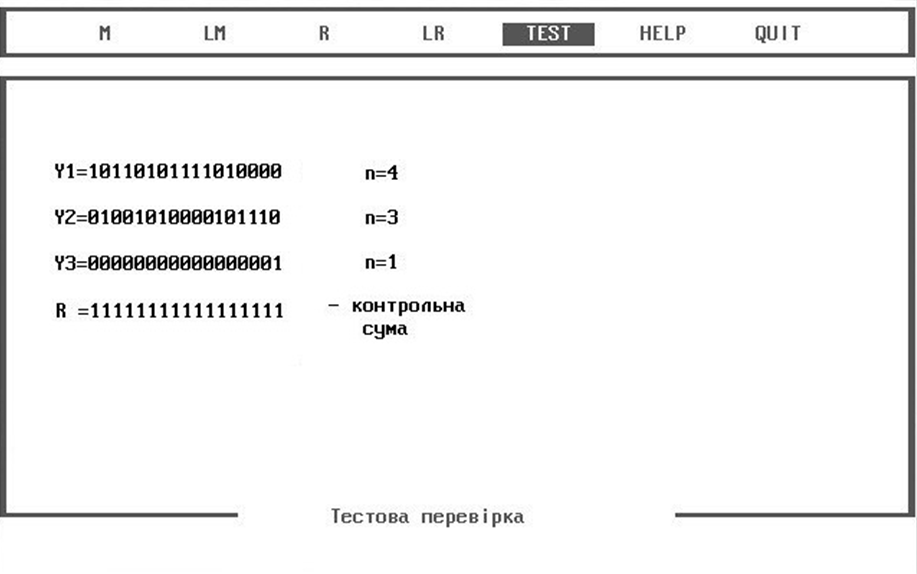
\includegraphics[width = \linewidth]{./assets/00-bw.png}
				\caption{}
				\label{subfig:mikrokod-result-00}
				\end{subfigure}
				\quad
				\begin{subfigure}[t]{0.5\linewidth - 1em}
				\centering
					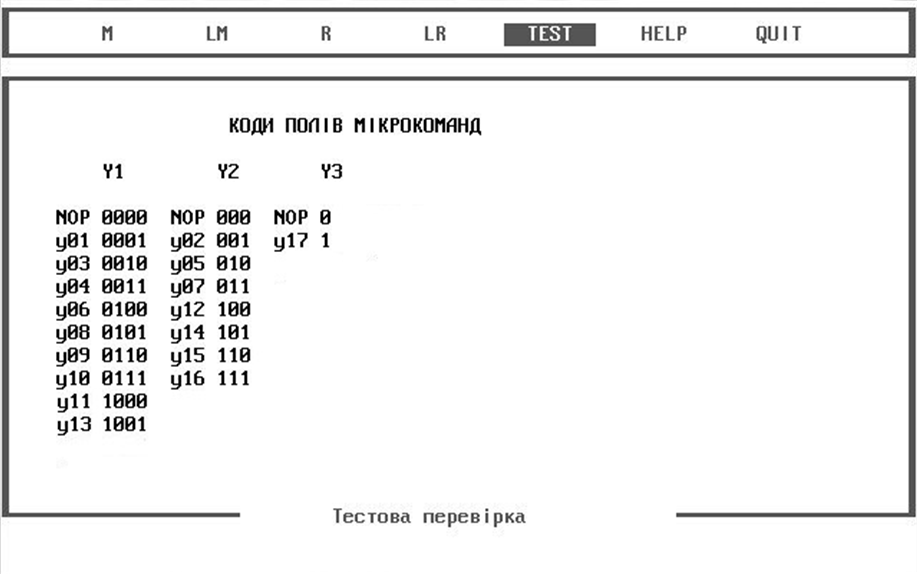
\includegraphics[width = \linewidth]{./assets/01-bw.png}
				\caption{}
				\label{subfig:mikrokod-result-01}
				\end{subfigure}
			\caption{Результат обробки початкових даних програмою «Мікрокод»: \subref{subfig:mikrokod-result-00}~— матриця включення та контрольна сума, \subref{subfig:mikrokod-result-01}~— результат кодування мікрооперацій за множинами}
			\label{fig:mikrokod-result}
			\end{figure}
			
	\section{Висновок}
		Під час виконання даної лабораторної роботи ми закріпили теоретичні знання з синтезу керуючих автоматів з програмованою логікою, навчились синтезувати мікрокоманди, будувати закодовану мікропрограму та розробляти структурну схему керуючого автомата з програмованою логікою.
\end{document}
